
%
% Chapter 6
%

\chapter{Future Work}

Throughout the course of this experiment, there have been a variety of areas that were adjusted to try and optimize the data. In this chapter, continued work and optimizations for future experiments are discussed.

\section{Detector Upgrades}

In a given experiment, the detectors are one of the single most important pieces of equipment. Two different styles of HPGe detectors were used, to varying success, and different magnetic configurations were used to optimize efficiency. Further steps are being taken for the future of conversion electron experiments at Notre Dame in both areas.

\subsection{fIREBAll}

The La Crosse \textbf{I}nternal Conve\textbf{R}sion \textbf{E}lectron \textbf{B}all \textbf{A}rray (fIREBAll) will be the next generation of ICEBall[FIGURE OUT CITATION]. The Major Research Instrumentation (MRI) proposal to the National Science Foundation (NSF) for funding has been approved. The University of Wisconsin-La Crosse submitted the proposal. The ICEBall beamline at the NSL will become the fIREBAll beamline. The focus of the proposal was detector upgrades, both for the Si(Li) detectors, and the HPGe detectors.

With this proposal, there will be dedicated HPGe detectors for the array, with two Bizmuth Germanate (BGO) anti-Compton suppression shields. The current Si(Li) detectors would be replaced with two Si(Li) detectors, for a total of twelve detectors each. There would still be six detection planes, as the Si(Li) detectors would be stacked in a telescope formation, to allow for the measurement of higher energy E0 transitions. The current Si(Li) detectors in use are 5 $mm$ thick. All of the new detectors would be 5 $mm$ thick, making for an active stopping depth of 10 $mm$ when stacked. Additionally, the detectors would be 800 $mm^2$ surface area instead of 750 $mm^2$ of the current detectors. Over the past 25 years of use, the current Si(Li) detectors have begun to deteriorate. As seen in Figure \ref{fig:bad_sili}. There is a clear decline in the resolution of the detector between the different experiments.

\begin{figure}[!]
    \centering
    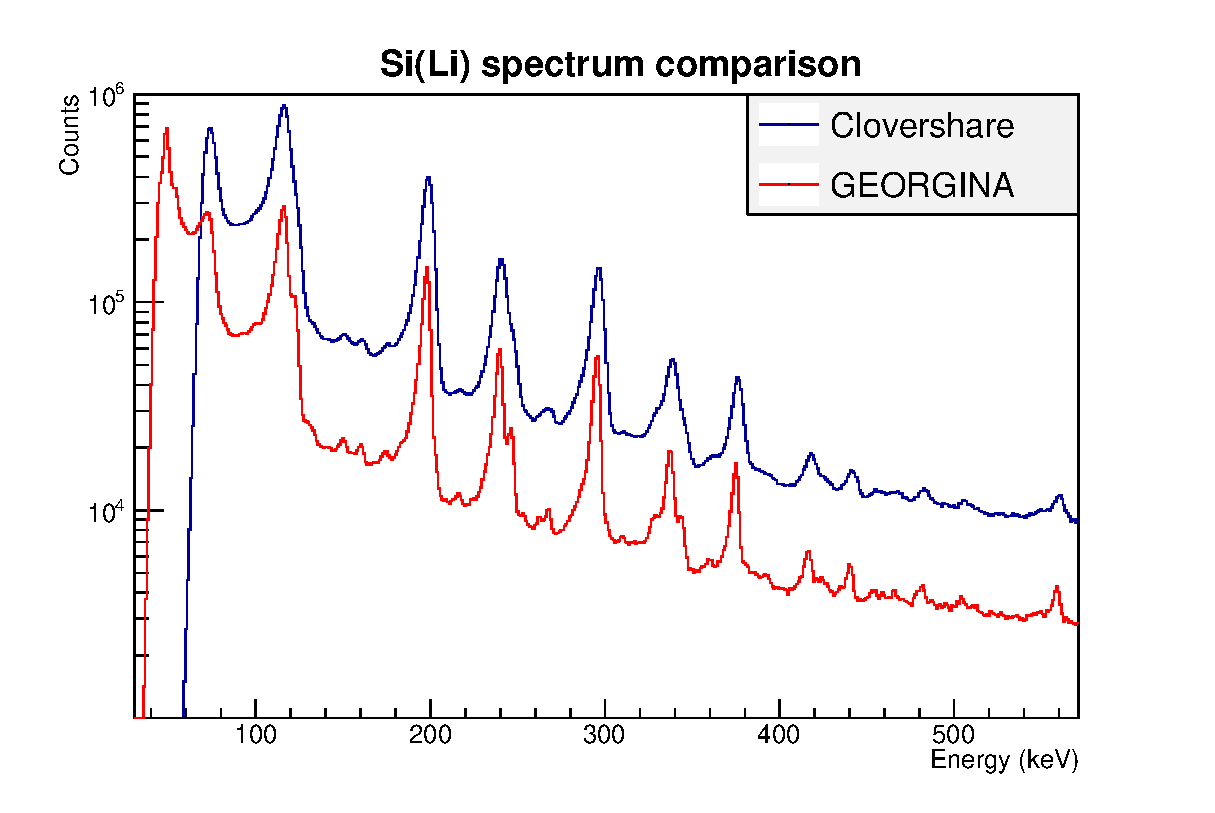
\includegraphics[scale=0.6]{Future_Figs/ResolutionComparison.eps}
    \caption{A comparison of the singles spectrum of one Si(Li) detector between the GEORGINA and Clovershare experiments. The resolution of the Si(Li) detector has deteriorated between the two experiments (the GEORGINA one was performed first). The LM peaks at \~{}240 keV and \~{}330 keV show this most clearly. The peaks are distinguishable in the GEORGINA data, but not in the Clovershare data.}
    \label{fig:bad_sili}
\end{figure}

\subsection{Magnet Designs}

To improve the detection efficiency of the conversion electrons, the magnetic configurations can be changed. This was done in the experiments to optimize for higher energies. When the original magnetic configurations were used, the permanent magnets used were 0.5 cm thick SmCo$_5$ squares. These thin squares are not, necessarily, creating the most optimal magnetic field.

Using GEANT4 [CITE] and [UHHHH?], a variety of magnetic shapes were modeled, varying the profile (square vs triangle) and the thickness. Two extremes would be chosen, with steps shifting between modelled, to find an optimal choice. The thickness was also varied between uniform and a gradient. [I NEED STUFF FROM KEVIN].

After 

\section{Target Upgrades}

One of the concerns and limitations of the original experiments was the thickness of the target. Ideally, the target being used would be less that 500 $\mu g/cm^2$, but the ones used were 1.7 $mg/cm^2$ and 1.44 $mg/cm^2$. While these targets were self-supporting, they were thick enough that electron straggling occurred, smearing out the spectrum.

To create a thinner target, it was decided to try and use a carbon-backing. The Sm was then evaporated onto the backing. The carbon was 20 $\mu g/cm^2$. In the targets made, the Sm was measured to be 170 $\mu g/cm^2$, ten times thinner than the original targets used.

To compare the old and new targets, an experiment was run with both targets inside of ICEBall. 

The new targets could be run with higher beam currents to get similar rates in the detectors, at what appeared to be a proportional rate to the target thickness.

At lower electron energies, the carbon-backed targets had far better resolution, as seen in Figure \ref{fig:target_test}.

\begin{figure}
    \centering
    \includegraphics[scale=0.3]{Future_Figs/SiLi3.png}
    \caption{Comparison of the thick (self-supporting) and thin (carbon-backed) targets. The spectra were taken during the same experiment. At low energies, the resolution is better in the thin target. Further, the energies of the peaks shift based on which target it is. This spectrum is not energy calibrated.}
    \label{fig:target_test}
\end{figure}

\begin{figure}
    \centering
    \includegraphics[scale=0.4]{Future_Figs/run005_triggerlive.eps}
    \caption{Trigger rate of the background with respect to time, after running on one of the carbon-backed targets. There is a clear indication of an exponential decay.}
    \label{fig:O15decay}
\end{figure}

\section{Electronics}

\section{Alternative Reactions}
